\documentclass{article}
\usepackage {inputenc, fullpage, listings, amsmath, graphicx, amssymb, xcolor}

\parindent 0pt

\title{%
   ECE 260: Continuous-Time Signals and Systems\\
    \Large Alex Holland - A01\\
    Assignment 2A\\
    }
\date{}

\begin{document}

\maketitle


2.1 {\bf [notation]}\\
(a)
\begin{equation*}
\begin{split}
    \mathcal{H}x(t) &= t^2 + 1\\
    (\mathcal{H}x)(t) &= [(t)^2] + 1\\
\end{split}
\end{equation*}

(b)
\begin{equation*}
\begin{split}
    & \mathcal{G} \mathcal{H} y (t) \\
    & [\mathcal{G}(\mathcal{H} y)](t)\\
\end{split}
\end{equation*}

(c)
\begin{equation*}
\begin{split}
    & \mathcal{H}x + y\\
    & (\mathcal{H}x) + y\\
\end{split}
\end{equation*}

(d)
\begin{equation*}
\begin{split}
    & x\mathcal{H} \mathcal{G}y\\
    & (x)[\mathcal{H} (\mathcal{G}y)]\\
\end{split}
\end{equation*}


2.2 {\bf [notation]}\\

(a)
the output of system $\mathcal{H}$ when its input is y:
\begin{equation*}
\begin{split}
    \mathcal{H}y
\end{split}
\end{equation*}

(b)
the output of system $\mathcal{H}$ evaluated at $2t - 1$ when the input to the system is $x$:
\begin{equation*}
\begin{split}
    \mathcal{H}x(2t - 1)
\end{split}
\end{equation*}

(c)
the output of system $\mathcal{H}$ evaluated at $t$ when the input to the system is $ax$:
\begin{equation*}
\begin{split}
    \mathcal{H}\{ax\}(t)
\end{split}
\end{equation*}

(d)
the output of system $\mathcal{H}$ evaluated at $5t$ when the input to the system is $x + y$:
\begin{equation*}
\begin{split}
    \mathcal{H}\{x + y\}(5t)
\end{split}
\end{equation*}

(e)
the derivative of the output of the system $\mathcal{H}$ when its input is $ax$:
\begin{equation*}
\begin{split}
    \mathcal{D}\mathcal{H}(ax)
\end{split}
\end{equation*}

(f)
the output of the system $\mathcal{H}$ when its input is the derivative of $ax$:
\begin{equation*}
\begin{split}
    \mathcal{H}\mathcal{D}(ax)
\end{split}
\end{equation*}

(g)
the sum of: 1) the output of the system $\mathcal{H}$ when its input is $x$; and 2) the output of the system $\mathcal{H}$ when its input is y:
\begin{equation*}
\begin{split}
    \mathcal{H}x + \mathcal{H}y
\end{split}
\end{equation*}

(h)
the output of the system $\mathcal{H}$ when its input is $x + y$:
\begin{equation*}
\begin{split}
    \mathcal{H}(x + y)
\end{split}
\end{equation*}

(i)
the derivative of $x$ evaluated at $5t - 3$:
\begin{equation*}
\begin{split}
    \mathcal{D}x (5t - 3)\\
\end{split}
\end{equation*}


\bigbreak
3.1 {\bf [time/amplitude transformations]}\\
(f)\\
$y(t) = x(7[t + 3])$\\
We must do the following transformations:
\begin{enumerate}
  \item  time shift left by 21
  \item time scale by compressing horizontally by a factor of 7
\end{enumerate}  
  
  
\bigbreak
3.2 {\bf [time transformation]}\\
$x_2(t)$ is generated from $x_1(t)$ from the following transformations:
\begin{enumerate}
  \item time shift left by 1
  \item time scaling by 4
  \item time reversal
\end{enumerate}  
Which we can represent as:
\begin{equation*}
\begin{split}
    x_2(t) = x_1(-4t - 1)
\end{split}
\end{equation*}


\bigbreak
3.4 {\bf [time/amplitude transformations]}\\
(a)
\begin{center}
    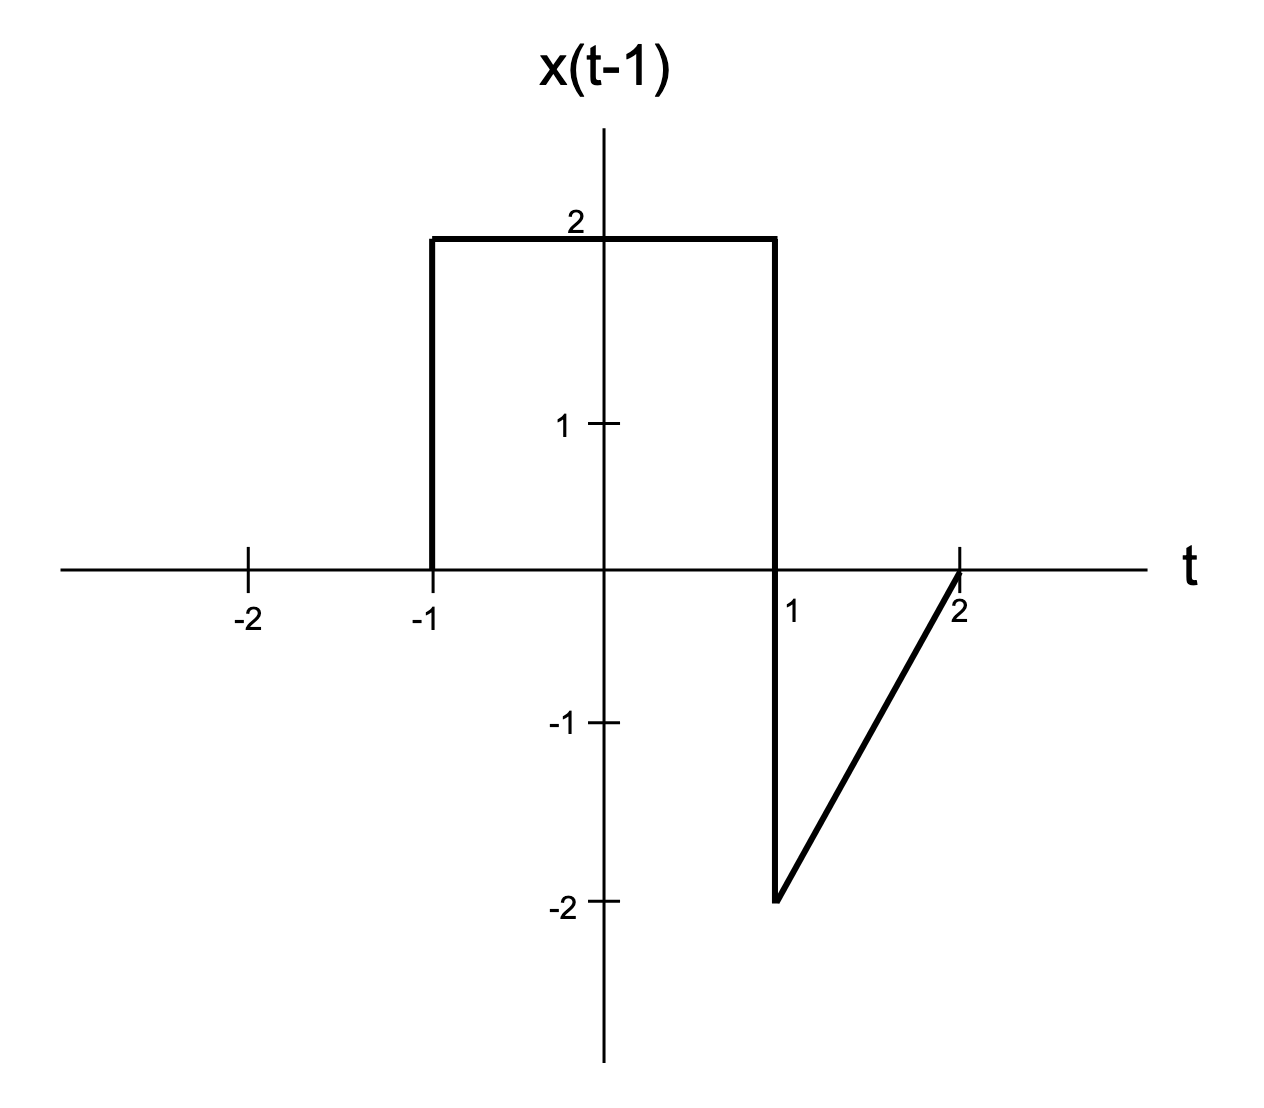
\includegraphics[width=0.5\textwidth]{34a.png}
\end{center}

(b)
\begin{center}
    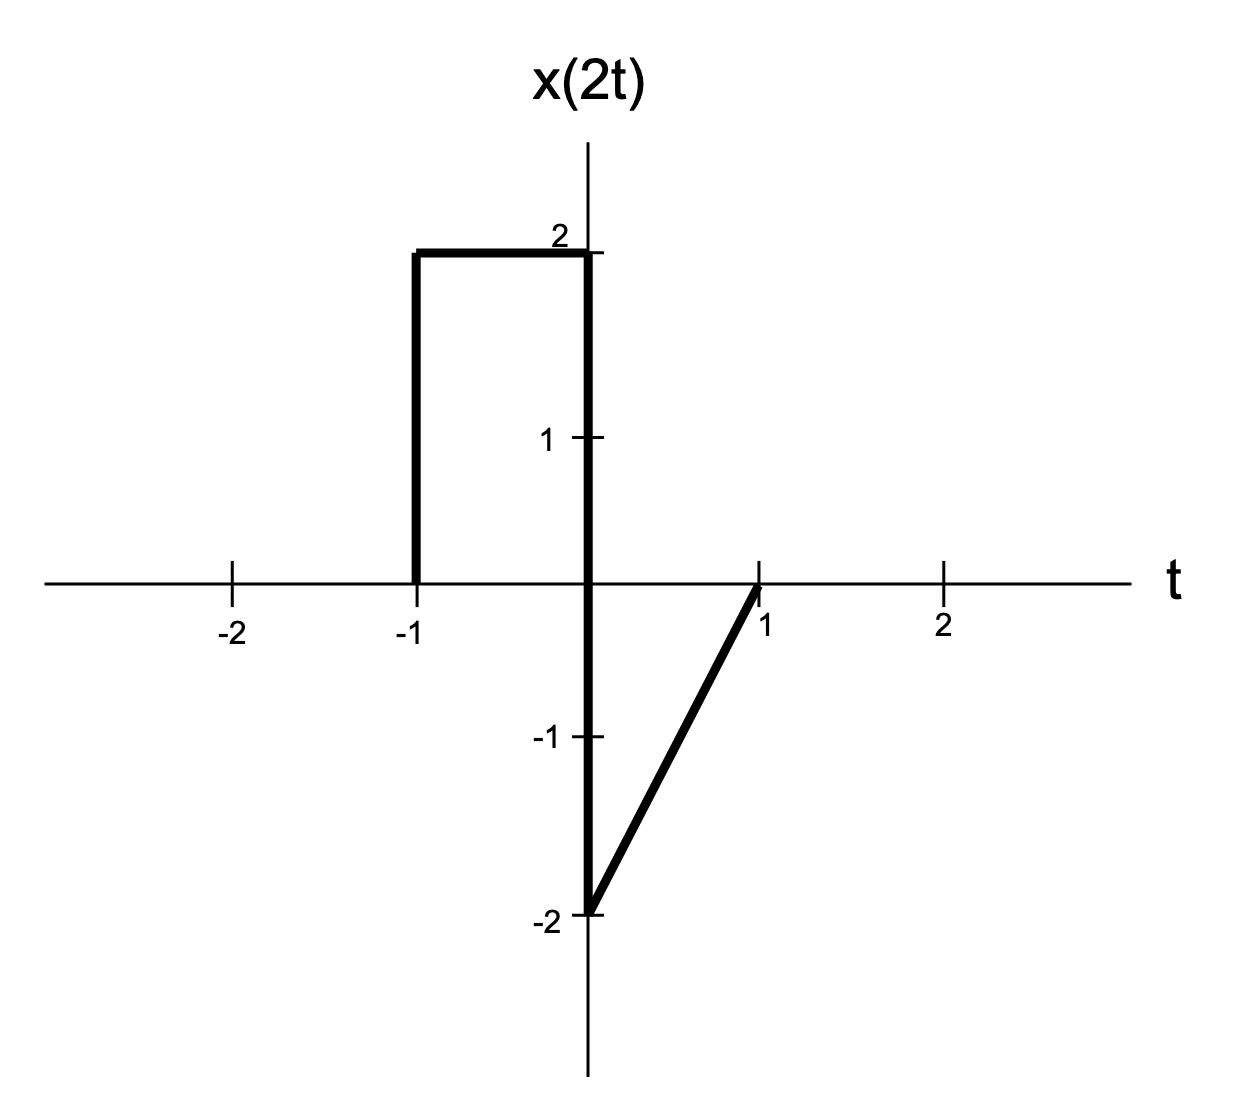
\includegraphics[width=0.5\textwidth]{34b.png}
\end{center}

(c)
\begin{center}
    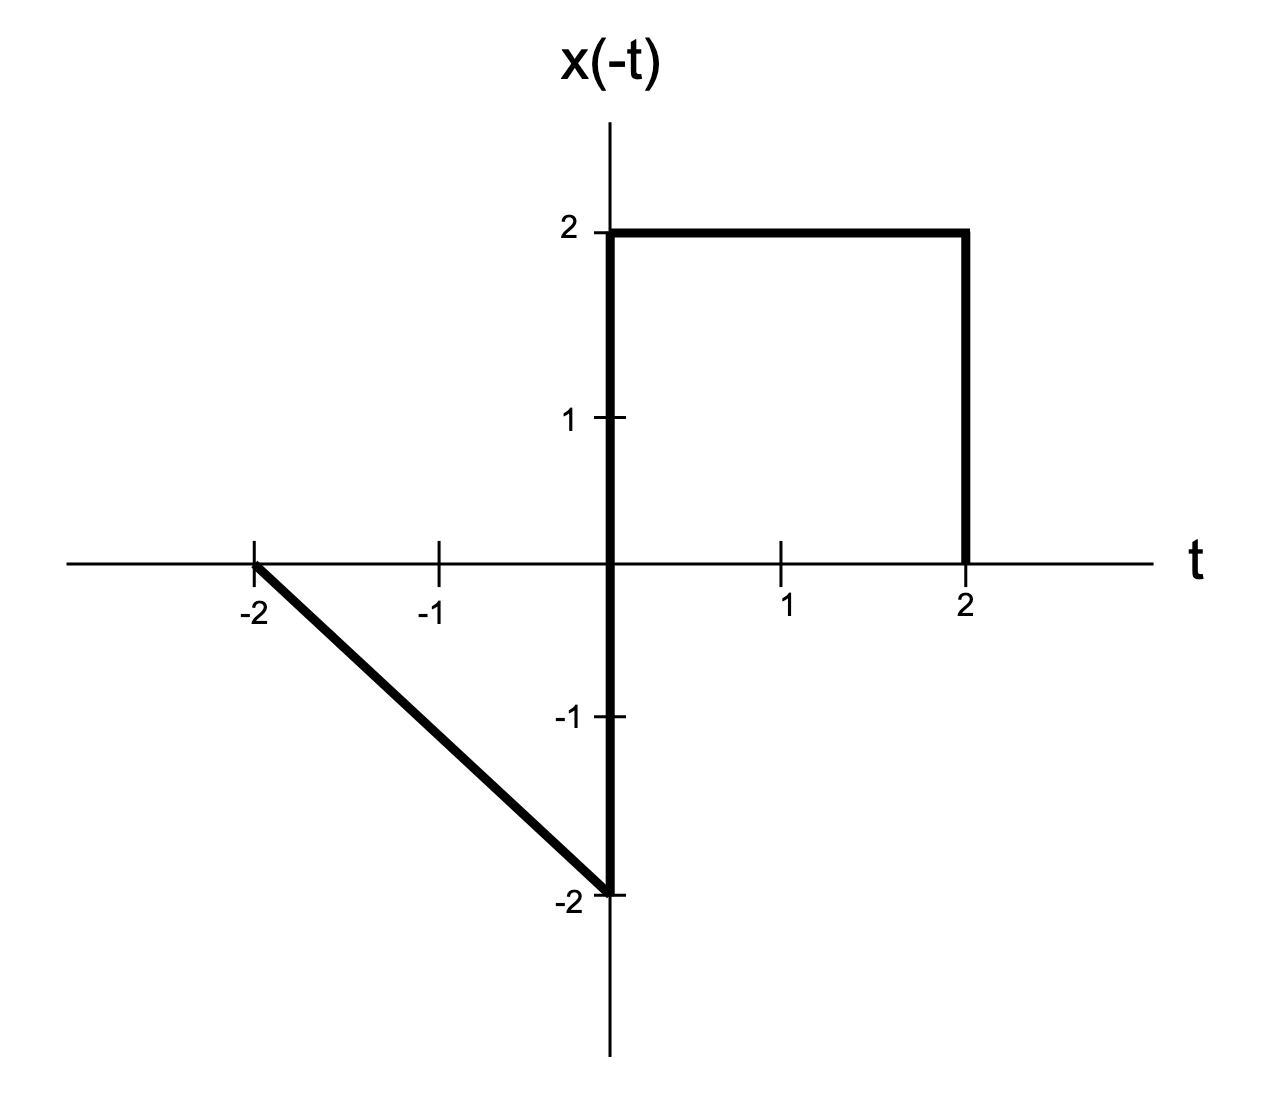
\includegraphics[width=0.5\textwidth]{34c.png}
\end{center}

(d)
\begin{center}
    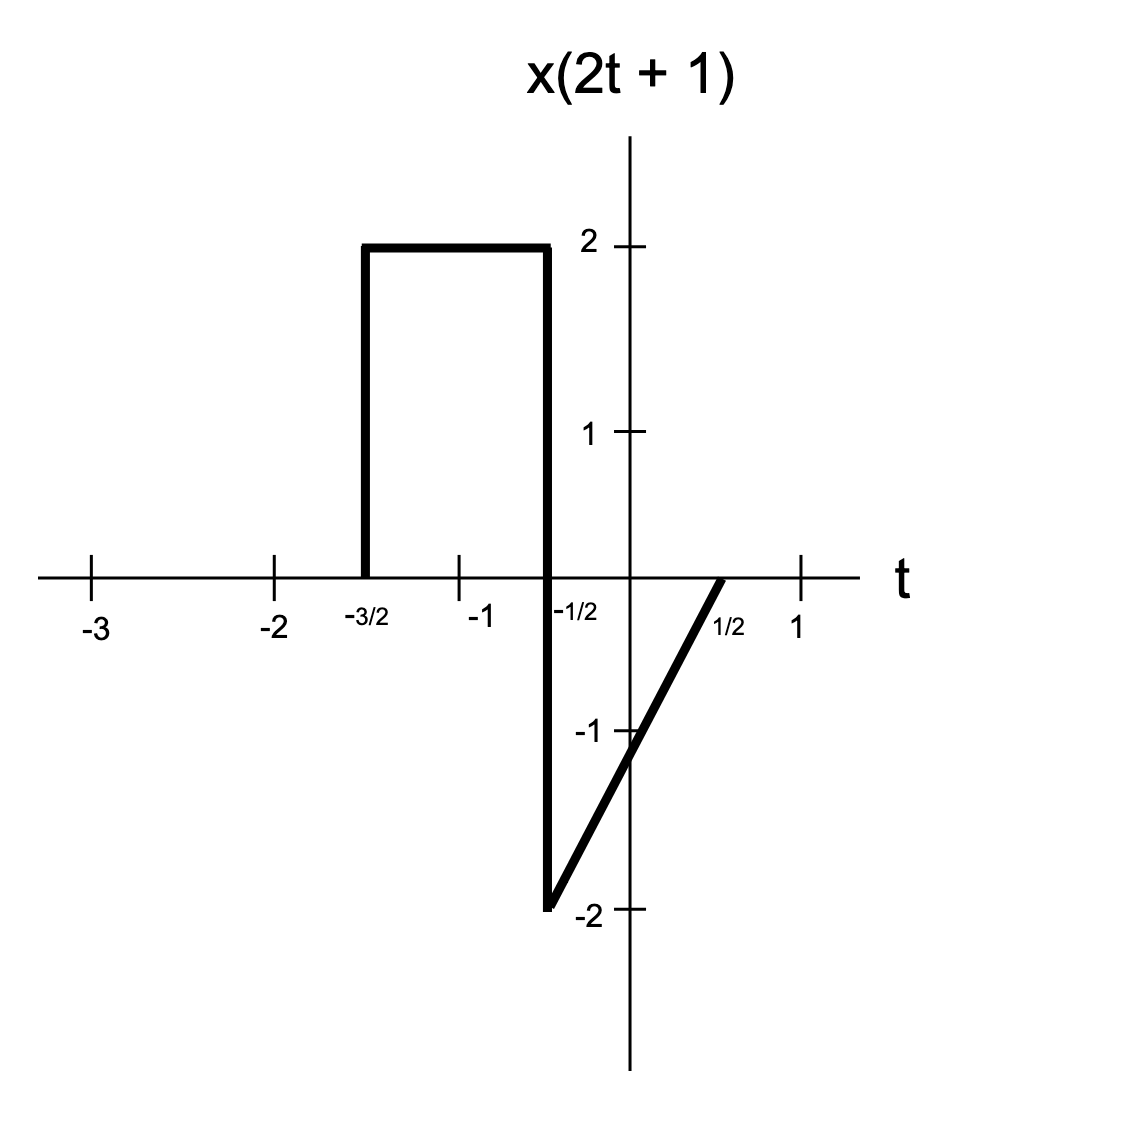
\includegraphics[width=0.5\textwidth]{34d.png}
\end{center}


\bigbreak
3.6 {\bf [periodicity]}\\
(e)
\begin{equation*}
\begin{split}
    x(t) &= cos(14t - 1) + cos(77t - 3)\\
    T_1 &= \frac{2\pi}{14}\\
    T_2 &= \frac{2\pi}{77}\\
    \frac{T_1}{T_2} &= \frac{\frac{2\pi}{14}}{\frac{2\pi}{77}}\\
    &= \frac{11}{2}
\end{split}
\end{equation*}
$\therefore$ the function $x$ is periodic and $T = 2T_1 = \frac{2 \pi}{7}$\\

(f)
\begin{equation*}
\begin{split}
    x(t) &= cos(et) + sin(42t)\\
    T_1 &= \frac{2\pi}{e}\\
    T_2 &= \frac{2\pi}{42}\\
    \frac{T_1}{T_2} &= \frac{\frac{2\pi}{e}}{\frac{2\pi}{42}}\\
    &= \frac{42}{e}\\
\end{split}
\end{equation*}
$\frac{42}{e}$ is irrational $\therefore$ the function $x$ is not periodic\\

(g)
\begin{equation*}
\begin{split}
    x(t) &= |sin(\pi t)|\\
    T &= \frac{2\pi}{\pi}\\
    &= 2
\end{split}
\end{equation*}
The absolute value of sine cut's the period in half.\\
\begin{equation*}
\begin{split}
    T &= \frac{2}{2}\\
    &= 1\\
\end{split}
\end{equation*}
$\therefore$ the function $x$ is periodic and $T = 1$\\


\bigbreak
3.9 {\bf [even/odd symmetry]}\\
(c)
\begin{equation*}
\begin{split}
    x(t) &= |t^3|\\
    x(t) &= x(-t)\\
    |t|^3 &= |-t|^3\\
    t^3 &= t^3\\
\end{split}
\end{equation*}
$\therefore$ the function is even\\

(d)
\begin{equation*}
\begin{split}
    x(t) &= cos(2 \pi t) sin(2 \pi t)\\
    x(-t) &= (cos 2 \pi(-t))(sin 2 \pi(-t))\\
    &= cos 2\pi t(-sin2 \pi t)\\
    &= -cos(2 \pi t) sin (2 \pi t)\\
\end{split}
\end{equation*}
$\therefore$ the function is odd\\


\bigbreak
3.10 {\bf [symmetry and sums/products]}\\
(b)\\
We want to prove that the sum of two odd functions is odd.\\
Let $x_1(t)$ and $x_2(t)$ be odd functions.
\begin{equation*}
\begin{split}
    x_1(-t) &= -x_1(t)\\
    x_2(-t) &= -x_2(t)\\\\
    (x_1 + x_2)(t) &= x_1(t) + x_2(t)\\
    (x_1 + x_2)(-t) &= x_1(-t) + x_2(-t)\\
    &= -x_1(t) - x_2(t)\\
    &= -(x_1 + x_2)(t)\\
\end{split}
\end{equation*}
$\therefore$ the sum of two odd functions is odd.


\bigbreak
3.17 {\bf [even/odd decomposition, signal properties]}\\
\begin{equation*}
\begin{split}
    h_e(t) &= t[u(t) - u(t - 1)] + u(t - 1) \text{ for $t \geq 0$}\\
    &= tu(t) + (-t + 1) u (t - 1)\\
\end{split}
\end{equation*}
Since $h$ is causal and has the even part $h_e$ we can determine $h$ as follows:\\

Since $h_e(t)$ is even, for all $t < 0$:
\begin{equation*}
\begin{split}
    h_e(t) &= h_e(-t)\\
    & (-t)u(-t) + (t + 1) u (-t - 1)\\
\end{split}
\end{equation*}
 Since $h_o(t) = -h_e(t)$, then for $t < 0$:

\begin{equation*}
\begin{split}
    h_o(t) &= -h_e(t)\\
    &= -[(-t)u(-t) + (t + 1) u (-t - 1)]\\
    &= t u (-t) + (-t - 1) u (-t - 1)\\
\end{split}
\end{equation*} 
For $t < 0$ we can determine $h_o(t) = -h_e(t)$:

\begin{equation*}
\begin{split}
    h_o(t) &= -h_e(t)\\
    &= -[(-t) u (-t) + (t + 1) u (-t - 1)]\\
    &= t u (t) + (-t - 1) u (t - 1)\\
\end{split}
\end{equation*} 

$\therefore$ we can determine $h(t) = h_o(t) + h_e(t)$:
\begin{equation*}
\begin{split}
    h(t) &= h_o(t) + h_e(t)\\
    &= [tu(t) + (-t + 1) u (t - 1)] + [tu(t) + (-t + 1) u (t - 1)]\\
    &= (2t) [u(t) - u(t - 1)] + 2u(t - 1)\\
\end{split}
\end{equation*} 


\bigbreak
3.18 {\bf [signal properties]}\\
(b)
We are given the following properties regarding a function $x$:
\begin{itemize}
  \item $x(t) = t - 1$ for $0 \leq t \leq 1$;
  \item the function $v$ is casual, where $v(t) = x(t - 1)$; and
  \item the function $w$ is odd, where $w(t) = x(t) + 1$.
\end{itemize}
Since $v(t) = x(t - 1)$ is causal, we get
\begin{equation*}
\begin{split}
    v(t) &= 0 \text{ for $t < 0$}\\
    x(t - 1) &= 0 \text{ for $t < 0$}\\
    x(t) &= 0 \text{ for $t + 1 < 0$}\\
    x(t) &= 0 \text{ for $t < -1$}
\end{split}
\end{equation*} 

As stated, $w(t) = x(t) + 1$ is odd, so $x$ is shifted up by 1.\\

$\therefore$ we can conclude that the piecewise function $x(t)$ for all $t$ is

\begin{equation*}
\begin{split}
    &= \begin{cases}
        0 & t < -1\\
        t - 1 & -1 \leq t \leq 1\\
        -2 & t > 1
    \end{cases}\\
\end{split}
\end{equation*}


\bigbreak
3.20 {\bf [properties of delta functions]}\\
(a)
\begin{equation*}
\begin{split}
    \int_{-\infty}^{\infty} sin(2t + \frac{\pi}{4}) \delta(t) dt
    &= [sin(2t + \frac{\pi}{4}] \big|_{t=0} \\
    &= sin(\frac{\pi}{4})\\
    &= \frac{1}{\sqrt{2}}
\end{split}
\end{equation*}

(b)
\begin{equation*}
\begin{split}
    \int_{-\infty}^{t} cos(\tau) \delta (\tau + \pi) d\tau
    &= \begin{cases}
        cos(\tau) \big|_{t = -\pi} & \text{for $t > -\pi$}\\
        0 & \text{for $t < -\pi$}
    \end{cases}\\
    &= \begin{cases}
        cos(-\pi) & \text{for $t > -\pi$}\\
        0 & \text{for $t < -\pi$}
    \end{cases}\\
    &= \begin{cases}
        -1 & \text{for $t > -\pi$}\\
        0 & \text{for $t < -\pi$}
    \end{cases}\\
    &= -u(t + \pi)\\
\end{split}
\end{equation*}

(c)
\begin{equation*}
\begin{split}
    \int_{-\infty}^{\infty} x(t) \delta (at-b)dt, & \text{ where $a$ and $b$ are real constants and $a \neq 0$}\\
     &= \begin{cases}
        \int_{-\infty}^{\infty} x (\frac{\lambda}{a}) \delta(\lambda - b)(\frac{1}{a})d\lambda & \text{for $a > 0$}\\
        \int_{\infty}^{-\infty} x (\frac{\lambda}{a}) \delta(\lambda - b)(\frac{1}{a})d\lambda & \text{for $a < 0$}
    \end{cases}\\
     &= \begin{cases}
        \frac{1}{a} \int_{-\infty}^{\infty} x (\frac{\lambda}{a}) \delta(\lambda - b)d\lambda & \text{for $a > 0$}\\
        -\frac{1}{a} \int_{\infty}^{-\infty} x (\frac{\lambda}{a}) \delta(\lambda - b)d\lambda & \text{for $a < 0$}
    \end{cases}\\
    &= \frac{1}{|a|} \int_{-\infty}^{\infty} x (\frac{\lambda}{a}) \delta(\lambda - b)d\lambda\\
    &= \frac{1}{|a|} [x(\frac{\lambda}{a})]\big|_{\lambda = b}\\
    &= \frac{1}{|a|}x (\frac{b}{a})
\end{split}
\end{equation*}

(f)
\begin{equation*}
\begin{split}
    \int_{0}^{\infty} \tau^2 cos(\tau)\delta(\tau + 42) d\tau
    &= \int_{0}^{\infty} 0d\tau\\
    &= 0
\end{split}
\end{equation*}


\bigbreak
D.101 {\bf [MATLAB identifiers]}\\
(a)
$4ever$ - invalid, first character must be a letter\\
(b)
$\$rich\$$ - invalid, first character must be a letter\\
(c)
$foobar$ - valid\\
(d)
$foo\_bar$ - valid\\
(e)
$\_foobar$ - invalid, first character must be a letter\\


\bigbreak
D.106 {\bf [MATLAB expressions}\\
(a)
\begin{lstlisting}
    v = [0 1 2 3 4 5]
    2*v-3
    ans = -3 -1 1 3 5 7
\end{lstlisting}

(b)
\begin{lstlisting}
    v = [0 1 2 3 4 5]
    1./(v+1)
    ans = 1.0000 0.5000 0.3333 0.2500 0.2000 0.1667
\end{lstlisting}

(c)
\begin{lstlisting}
    v = [0 1 2 3 4 5]
    v.^5 - 3
    ans = -3 -2 29 240 1021 3122
\end{lstlisting}

(d)
\begin{lstlisting}
    v = [0 1 2 3 4 5]
    abs(v) + v.^4
    ans = 0 2 18 84 260 630
\end{lstlisting}


\end{document}
